\section{Motion Ambiguity and State Aliasing}
\label{sec:diagnosis}

As briefed in \cref{sec:introduction}, we observe two dominant failure modes recent VLA encounters when trained on dynamic tasks, both stemming from a Markovian assumption shared by every pretrained VLA today, where the current observation is treated as a sufficient context for inferring action. We illustrate each on our four dynamic tasks (setup in \cref{sec:exp-setup}).

\begin{figure}[!t]
	\centering
	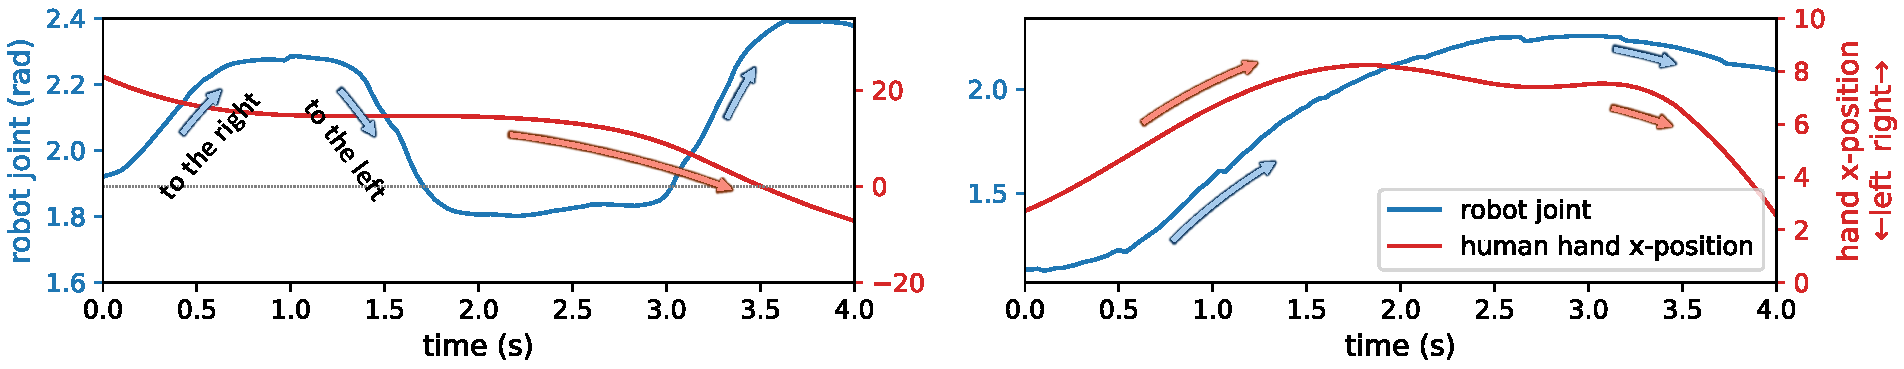
\includegraphics[width=0.9\columnwidth]{2026-corl-unveil-template/figures/jittery.pdf}
	\vspace{-1em}
	\caption{\textbf{Robot joint action (blue) does not track the human hand (red).} Side-by-side comparison of a Drop Catch rollout from the baseline (VLASH, left) and \ours~(right). The baseline oscillates left-to-right continuously while the human hand moves in a single direction, whereas \ours~closely tracks the hand.}
	\label{fig:jittery}
\end{figure}

\noindent\textbf{Motion ambiguity.}
A policy $\pi(o_t)$ conditioned on the current frame observes where objects are, but not where they are going. Recent works on dynamic tasks all focus on reducing inference latency, which lets $\pi$ act on a more recent observation, but does not inform the policy of object motion. \figref{fig:jittery} shows the resulting behavior on Drop Catch: when the policy is supposed to shadow human hand motion, the VLASH~\cite{vlash} policy instead produces actions that oscillate left-to-right. The same representational gap is also evident in our motion probe study in \cref{para:motion_probe}: linearly decoding object velocity from each baseline collapses on tasks where object motion is the only cue, with $R^2 \le 0.03$ on Flick Catch and $\le 0.09$ on Wine Pour (\cref{tab:motion_probe}). The policy has no basis for anticipating where a moving target will be.

\begin{wraptable}{r}{0.45\columnwidth}
\centering
\small
\setlength{\tabcolsep}{4pt}
\begin{tabular}{lcc}
\toprule
Method & Flick Catch & Wine Pour \\
\midrule
RTC~\cite{rtc} & 0\% & 0\% \\
VLASH~\cite{vlash} & 0\% & 0\% \\
\ours~(Ours) & \textbf{68\%} & \textbf{97.6\%} \\
\bottomrule
\end{tabular}
\caption{\textbf{Success on the untrimmed Flick Catch and Wine Pour}, where each episode retains the release-and-retract phase that produces state aliasing. Both asynchronous baselines fail every rollout; \ours\ completes the task by using \TEMPOACT\ to disambiguate phases the current frame cannot.}
\label{tab:state_alias}
\end{wraptable}

\noindent\textbf{State aliasing.}
A second failure mode arises from task structure and persists in the absence of motion. Multi-stage tasks force the policy to produce opposite actions from visually near-identical moments. For example, reaching for a plate at the start of a task and releasing it and pulling the gripper back look nearly the same from the head camera, but the corresponding future actions are opposite. The policy then hesitates between the two options: the gripper commits to neither, and the task fails to advance. Trained on the original Wine Pour and Flick Catch tasks, both asynchronous baselines fail every rollout ($0/50$; \cref{tab:state_alias}). To obtain nonzero baseline numbers for the main results in \cref{tab:success_rates}, we manually remove aliased state by trimming the release-and-retract phase from every training episode. Having to remove this segment at all is itself evidence of the failure for our baseline models.

\noindent\textbf{What the two failures require.}
Both failures come down to the same gap: a single frame carries no temporal context. To perceive scene motion, the policy needs a signal built from recent observations; to tell task phases apart, it needs a signal built from its own recent actions. Both signals summarize data the policy is already receiving at inference time.

%===============================================================================
